\documentclass[11pt]{article}
\usepackage{graphicx}
\usepackage{amsmath}
\usepackage{amssymb}
\usepackage{paralist}
\usepackage{subcaption}
\usepackage{floatrow}

\usepackage[margin=1in]{geometry}
\newcommand{\set}[1]{\mathcal{#1}}
\newcommand{\material}{\mathcal{M}}
\newcommand{\fe}{\mathcal{E}}
\usepackage{array}
\newcolumntype{L}[1]{>{\raggedright\let\newline\\\arraybackslash\hspace{0pt}}m{#1}}
\newcolumntype{C}[1]{>{\centering\let\newline\\\arraybackslash\hspace{0pt}}m{#1}}
\newcolumntype{R}[1]{>{\raggedleft\let\newline\\\arraybackslash\hspace{0pt}}m{#1}}

\title{ \large{Massachusetts Institute of Technology\\~\\
	Department of Electrical Engineering and Computer Science\\~\\~\\
	Proposal for Thesis Research in Partial Fulfillment\\~\\
	of the Requirements for the Degree of\\~\\
	Doctor of Philosophy }}
\date{}
\begin{document}
	\pagenumbering{gobble}
	\maketitle
\begin{flushleft}
 Title: Multiscale Methods for Fabrication Design\\~\\

\begin{tabular}{L{4cm} p{6cm} p{8cm}}
\hskip-0.2cm Submitted by: & Desai Chen & \underline{\hspace{6cm}}\\
              &32 Vassar St., 32-311 & (Signature of author) 	  \\
              &Cambridge, MA 02139&
\end{tabular}\\~\\

Date of submission: May , 2016\\~\\
Expected date of completion: June 2016\\~\\
Laboratory where thesis will be done: MIT CSAIL\\~\\
Brief statement of the problem:\\~\\
Crafting the behavior of a deformable object is difficult---whether it is a biomechanically accurate character model or a multimaterial 3D print design.
Getting it right requires constant iteration, performed either manually or driven by an automated system.
Throughout this process the geometry and material composition of the object are in constant flux.
Accurate simulation of deformable objects using standard finite element methods is computationally expensive especially for large deformations beyond linear elasticity regime.
We propose to speed up simulation using multiscale methods that approximates the solution at coarser scales while capturing the overall behavior with sufficient accuracy for design tasks.
\end{flushleft}
\newpage
\begin{center}
	MASSACHUSETTS INSTITUTE OF TECHNOLOGY\\
	Department of Electrical Engineering and Computer Science\\
	Cambridge, Massachusetts 02139\\~\\
	\textbf{Doctoral Thesis Supervision Agreement}\\~\\
\end{center}
\begin{tabular}{p{2cm} p{10cm}}
	To: & Department Graduate Committee \\
	From: & Dr. Wojciech Matusik, Thesis Supervisor
\end{tabular}\\~\\
The program outlined in the proposal\\~\\
\begin{tabular}{p{2cm} l}
	Title: & Multiscale Methods for Fabrication Design\\
	Author: & Desai Chen\\
	Date : & May 7, 2017
\end{tabular}\\~\\
is adequate for a Doctoral thesis. I believe that the appropriate readers for this thesis are\\~\\
\begin{tabular}{p{2cm} l}
	Reader 1: & Dr.\\
	Reader 2: & Dr.\\
	Reader 3: & Dr.
\end{tabular}\\~\\
Facilities and support for the research outlined in the proposal are available.
I am willing the supervise the research and evaluate the thesis report.\\~\\
\begin{flushright}
	\begin{tabular}{l l}
		Signature: & \underline{\hspace{6cm}}\\~\\
		Title: & \underline{\hspace{6cm}}\\~\\
		Date: & \underline{\hspace{6cm}}\\~\\
	\end{tabular}
\end{flushright}
Comments:
\newpage
\begin{center}
	MASSACHUSETTS INSTITUTE OF TECHNOLOGY\\
	Department of Electrical Engineering and Computer Science\\
	Cambridge, Massachusetts 02139\\~\\
	\textbf{Doctoral Thesis Supervision Agreement}\\~\\
\end{center}
\begin{tabular}{p{2cm} p{10cm}}
	To: & Department Graduate Committee \\
	From: & Dr. , Thesis Reader
\end{tabular}\\~\\
The program outlined in the proposal\\~\\
\begin{tabular}{p{4cm} l}
	Title: & Multiscale Methods for Fabrication Design\\
	Author: & Desai Chen\\
	Date : & May 7, 2017 \\
	Thesis Supervisor: & Dr. Wojciech Matusik\\
	Other Reader: & Dr.\\
	Other Reader: & Dr.
\end{tabular}\\~\\
is adequate for a Doctoral thesis. I am willing to aid in guiding the research and in
evaluating the thesis report as a reader.\\~\\
\begin{flushright}
	\begin{tabular}{l l}
		Signature: & \underline{\hspace{6cm}}\\~\\
		Title: & \underline{\hspace{6cm}}\\~\\
		Date: & \underline{\hspace{6cm}}\\~\\
	\end{tabular}
\end{flushright}
Comments:
\newpage
\begin{center}
	MASSACHUSETTS INSTITUTE OF TECHNOLOGY\\
	Department of Electrical Engineering and Computer Science\\
	Cambridge, Massachusetts 02139\\~\\
	\textbf{Doctoral Thesis Supervision Agreement}\\~\\
\end{center}
\begin{tabular}{p{2cm} p{10cm}}
	To: & Department Graduate Committee \\
	From: & Dr. , Thesis Reader
\end{tabular}\\~\\
The program outlined in the proposal\\~\\
\begin{tabular}{p{4cm} l}
	Title: & Multiscale Methods for Fabrication Design\\
	Author: & Desai Chen\\
	Date : & May 7, 2017 \\
	Thesis Supervisor: & Dr. Wojciech Matusik\\
	Other Reader: & Dr.\\
	Other Reader: & Dr.
\end{tabular}\\~\\
is adequate for a Doctoral thesis. I am willing to aid in guiding the research and in
evaluating the thesis report as a reader.\\~\\
\begin{flushright}
	\begin{tabular}{l l}
		Signature: & \underline{\hspace{6cm}}\\~\\
		Title: & \underline{\hspace{6cm}}\\~\\
		Date: & \underline{\hspace{6cm}}\\~\\
	\end{tabular}
\end{flushright}
Comments:
\newpage
\begin{center}
	MASSACHUSETTS INSTITUTE OF TECHNOLOGY\\
	Department of Electrical Engineering and Computer Science\\
	Cambridge, Massachusetts 02139\\~\\
	\textbf{Doctoral Thesis Supervision Agreement}\\~\\
\end{center}
\begin{tabular}{p{2cm} p{10cm}}
	To: & Department Graduate Committee \\
	From: & Dr. , Thesis Reader
\end{tabular}\\~\\
The program outlined in the proposal\\~\\
\begin{tabular}{p{4cm} l}
	Title: & Multiscale Methods for Fabrication Design\\
	Author: & Desai Chen\\
	Date : & May 7, 2017 \\
	Thesis Supervisor: & Dr. Wojciech Matusik\\
	Other Reader: & Dr.\\
	Other Reader: & Dr.
\end{tabular}\\~\\
is adequate for a Doctoral thesis. I am willing to aid in guiding the research and in
evaluating the thesis report as a reader.\\~\\
\begin{flushright}
	\begin{tabular}{l l}
		Signature: & \underline{\hspace{6cm}}\\~\\
		Title: & \underline{\hspace{6cm}}\\~\\
		Date: & \underline{\hspace{6cm}}\\~\\
	\end{tabular}
\end{flushright}
Comments:
\newpage
\pagenumbering{arabic}
\section{Introduction}
Objects with high-resolution, heterogeneous material properties are everywhere:
from the output of multimaterial 3D printers 
to virtual characters gracing the screen in summer blockbusters.
Designing such objects is made possible by the tight coupling of design
tools and numerical simulation which allows designers 
(or optimization algorithms) to update geometry or material parameters 
and subsequently estimate the physical effects of the change.
Fast, accurate simulation techniques that can handle runtime changes 
in geometry and material composition are a necessity for such iterative design algorithms.
The gold standard technique for estimating the mechanical behavior
of a deformable object under load is the finite element method (FEM).
While accurate, FEM is notoriously slow,
making it a major bottleneck in the iterative design process.
For this reason, there have been a large number of works on speeding up FEM simulations,
and these speed improvements have enabled FEM to be used in many performance critical tasks
such as computer animation, surgical training, and virtual/augmented reality.
Unfortunately, even though techniques such as model reduction or numerical coarsening 
can achieve order-of-magnitude performance increases,
they require expensive precomputation phases, typically on the order of minutes
for large meshes. This precomputation requires knowledge of an object’s 
geometry and material composition a priori,
something that is not known during a design task.
When the user updates the model by changing the geometry or the material distribution,
the preprocessing step must be run again.
Since this step is inside the design loop,
the user cannot get rapid feedback on the changes made to the object.
Additionally, many existing methods assume the object only undergoes small deformations
with known boundary conditions.
Extensions of these methods to large deformations with varying boundary conditions
severely increase the algorithm complexity and quickly diminishes the performance improvements.

We propose coarsening algorithms based on standard FEM
without introducing new types of spatial discretization which increases
algorithmic complexity.
Our algorithm reduces the element count by using coarser elements with data-driven
material properties suitable for design tasks.
The data is acquired before design iterations either from high-resolution simulations or from measurements.
At runtime, precomputed element material properties are applied to a coarse discretization.
The coarsened FEM models can accommodate varying geometry,
material assignments and boundary conditions of an elastic object.
We will fabricate exemplar objects and design physics experiments to validate that our coarsened approximations are sufficiently predictive of object behaviors.
An overview of the pipeline is shown in figure~\ref{fig:overview}.
\begin{figure}[ht]
	\centering
	\subcaptionbox{\label{fig:typical}Typical methods}{
		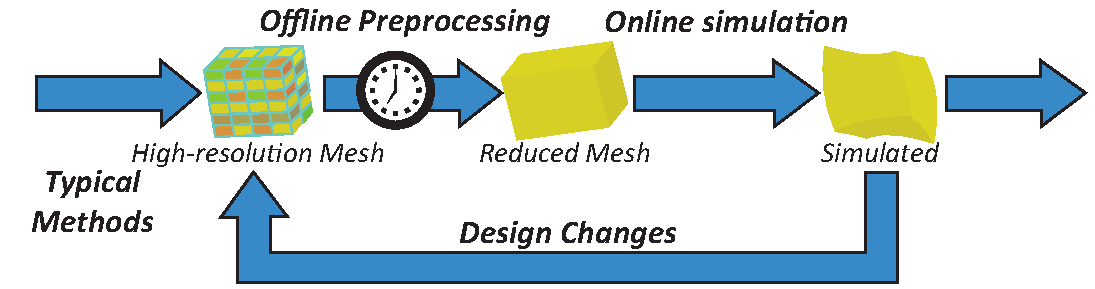
\includegraphics[width=0.7\columnwidth]{images/typical1.pdf}
	}
	\subcaptionbox{\label{fig:ours}Our method}{
		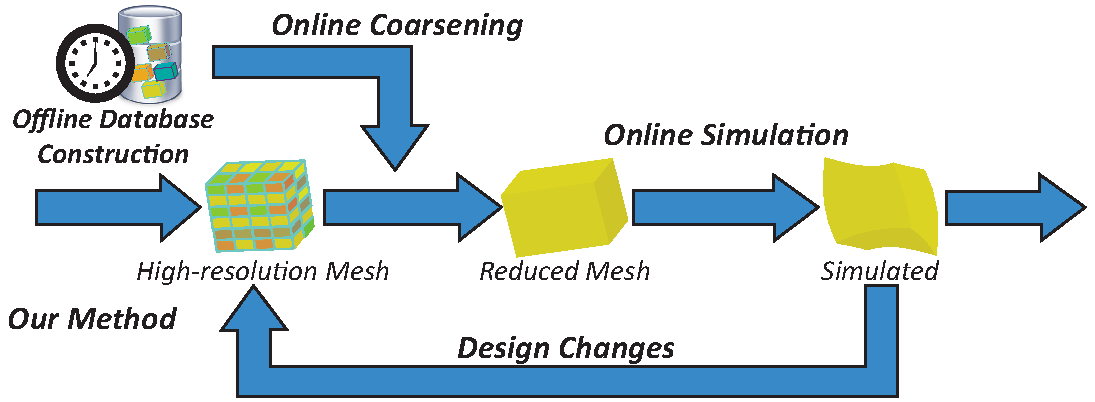
\includegraphics[width=0.7\columnwidth]{images/typical2.pdf}
	}
	\caption{
		(a) In a typical method, the preprocessing step of reducing element count is performed for every design change, making the design loop slow.
		(b) In our method, we move the time-consuming offline computation outside of the design loop.
	}
	\label{fig:overview}
\end{figure}

\section{Related Work}
Efficient FEM simulation plays an important role in designing deformable objects.
As mentioned, these problems are common in engineering and
graphics~\cite{bendsoe2004topology,Bickel2010,Kou2012,Skouras2013,Chen2013,Xu2014}.
We can broadly partition the space of approaches for optimizing FEM simulation into two categories.
We term the first category \emph{numerical} approaches.
These methods use fast matrix inversion techniques and other insights about the algebra of the finite element method to increase its performance.
Simulators based on the multigrid method~\cite{Peraire1992,Zhu2010,McAdams2011} and Krylov subspace techniques~\cite{Patterson2012} have yielded impressive performance increases.
Other hierarchical numerical approaches, as well as highly parallel techniques, have also been applied to improve the time required to perform complex simulations~\cite{Farhat1991,Mandel1993}.
Finally, Bouaziz et al.~\cite{Bouaziz:2014} propose specially designed energy functions and an alternating time-integrator for efficient simulation of dynamics.

The second set of methods are \emph{reduction} approaches.
These algorithms attempt to intelligently decouple or remove degrees of freedom (DOFs) from the simulated system.
This leads to smaller systems resulting in a massive increase in performance, with some decrease in accuracy.
The proposed methods fall into this category.
Note, however, that numerical and reduction approaches need not be mutually exclusive.
For example, our algorithm may potentially be used as a preconditioner for a numerical approach. Algorithms based on reduction approaches mitigate the inevitable increase in error using one or more of three approaches: Adaptive remeshing, higher-order shape functions, or by adapting the constitutive model.

Adaptive remeshing alters the resolution of the simulation discretization in response to various metrics (stress, strain etc.).
Such methods seek to maintain an optimal number of elements and thus achieve reasonable performance.
Adaptive remeshing has proven useful for simulating thin sheets such as cloth~\cite{narain2012}, paper~\cite{narain2013}, as well as elastoplastic solids ~\cite{Wicke:2010} and solid-fluid mixtures~\cite{Clausen2013}.
More general basis refinement approaches have also been suggested~\cite{Debunne2001,Grinspun2002}.
While these methods do improve the performance of simulation algorithms, they have some drawbacks.
First, they often require complicated geometric operations which can be time consuming to implement.
Second, they introduce elements of varying size into the FEM discretization.
This can lead to poor numerical conditioning if not done carefully.
Finally, in order to maintain accuracy, it may still be necessary to introduce many fine elements, leading to slow performance.
Alternatively, one  can turn to P-Adaptivity for help.
This refers to adaptively introducing higher-order basis functions in order to increase accuracy during simulation~\cite{Szabo2004}.
Unfortunately, these methods suffer from requiring complicated mesh generation schemes and are not well-suited for iterative design problems.

An alternative approach to remeshing is to use higher order shape functions in order to more accurately represent the object's motion using a small set of DOFs.
Modal simulation techniques fall into this category~\cite{Shabana1991,Krysl2001,Barbic:subspace:2005}.
Substructuring ~\cite{Barbic2011} decomposes an input geometry into a collection of basis parts, performing modal reduction on each one. These basis parts can be reused to construct new global structures.
Other approaches involve computing physically meaningful shape functions as an offline preprocessing step.
For instance,  Nesme et al.~\cite{Nesme2009} compute shape functions based on the static configuration of a high resolution element mesh induced via a small deformation of each vertex.
Faure et al.~\cite{Gilles2011} use skinning transformations as shape functions to simulate complex objects using a small number of frames.
Gilles et al.~\cite{Faure2011} show how to compute material aware shape functions for these frame-based models, taking into account the linearized object compliance. Both Nesme et al.~\cite{Nesme2009} and Faure et al.~\cite{Faure2011} accurately capture material behavior in the linear regime, but, because their shape functions cannot change with the deformed state of the material, they do not accurately capture the full, non-linear behavior of an elastic object. Our non-linear metamaterials rectify this problem.
Computing material aware shape functions improves both the speed and accuracy of the simulation.
However, these methods require a precomputation step that assumes a fixed material distribution and geometry.
If the material distribution changes, these shape functions must be recomputed, and this becomes a bottleneck in applications that require constantly changing material parameters.  

The final coarsening technique involves reducing the degrees of freedom of a mesh while simultaneously augmenting the constitutive model at each element, rather than the shape functions.
Numerical coarsening is an extension of analytical homogenization which seeks to compute averaged material for heterogeneous structures ~\cite{guedes1990,farmer2002}.
Numerical coarsening, for instance, has been applied to linearly tetrahedral finite elements~\cite{Kharevych2009}.
These methods require an expensive precomputation step (a series of static solves) that must be repeated when the material content, or the geometry of an object changes.
%The deficits of such a simulation method, such as locking, are well documented~\cite{Ted2000,Muller2002}.
This holds these methods back from being suitable for iterative design problems. 

Recently, three methods have been introduced that are similar to ours in spirit.
Bickel et al.~\cite{Bickel2009} measured force-displacement to compute a spatially varying set of Young's moduli, interpolated in strain space.
Our work also involves learning new constitutive models for finite element methods with several key differences.
First, we present a more robust energy-based metamaterial model that does not require incremental loading during simulation.
Second, the previous work relies on captured data to build constitutive model, while we use a new sampling strategy that allows us to build our metamaterial model virtually.
This allows us to leverage large, high-performance compute clusters to speed up the process.
Finally, their work is completely geometry dependent---their computed material models cannot be transferred to new meshes.
Xu et al.~\cite{Xu2014} and Li et al.~\cite{Li2014} computed material distribution given user specified forces and displacements.
	They compute materials in a low-dimensional space of material modes to speedup and regularize the solution.
	However, their method requires a known geometry, and furthermore,
	users cannot control per-element material assignment.
	Rather than computing material distribution,
	our method supports user specified topology changes and material assignment.
	These features are important due to the design-centric nature of our work.

Data-driven techniques have also been applied to add fine detail to coarse surgical simulations \cite{Cotin1999,Kavan:2011,Seiler2012}. While these methods do not help with the type of iterative design problems addressed here, they could be combined with our fast coarsening in order to quickly ``upscale'' coarsened simulation results to original simulation resolution.
\section{Coarsening for Elastostatics}
In this study, we introduce data-driven finite elements (DDFEM) to 
improve the simulation speed at the cost of small inaccuracy for elastostatic problems with heterogeneous non-linear materials. DDFEM focuses on finite elements defined one a regular grid.
To handle irregular boundary geometry, we will apply the use embedded finite elements for partially filled elements.
Using regular elements enables trivial combination of fine elements into coarser blocks of elements. This operation can be applied hierarchically to coarsen a mesh multiple times.
In this section, we discuss the two main stages of DDFEM computation---offline metamaterial construction and online coarsening.

\paragraph{Material palettes and mappings}
This study focuses on designs made of a discrete set of materials. The methodology can be extended to handle continuous mixtures of materials.
We note that designers often do not work in a continuous space of materials but limit themselves to a relatively compact set (e.g. rubber, wood, steel) related to their problem domain. We call these discrete sets of materials palettes and denote them $\set{P}=\{\material_0, \material_1, \hdots, \material_n\}$. Here $\material_i$ denotes a specific material model in $\set{P}$, and $n$ is the size of the material palette. In this work we further limit ourselves to (nonlinear) hyper-elastic materials, which means that each $\material_i$ can be represented by a strain energy density function $V$.
We also include a void (or empty) material in every palette. This allows us to perform topology changes in the same manner in which we perform material assignment updates.
In subsequent sections, we use a left superscript to indicate the level of coarsening. For example, $\set{P}^0$ denotes a material palette at the fine scale while $\set{P}^1$ denotes the new palette of metamaterials that results from the first coarsening step.

\paragraph{Coarsening for finite elements}
The key component of our DDFEM is coarsening. It reduces the number of elements in a finite element simulation mesh in order to improve runtime performance. Since simply removing elements can greatly reduce the accuracy of the simulation, coarsening schemes assign new materials to coarsened elements to minimize this effect.
We regard the global coarsening of a simulation mesh as the result of many local coarsening operations which map from contiguous subsets of fine elements with applied materials to coarse elements with new, optimized materials.
Our goal is to precompute these fitted materials so that coarsening is fast at runtime.

Each local coarsening operation merges a 2x2 block of elements into a single coarse element (Figure~\ref{fig:coarsen}).
\begin{figure}
	\centering
	
	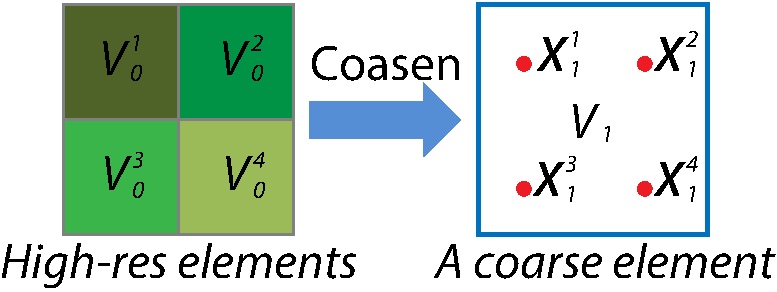
\includegraphics[width=0.5\textwidth]{images/coarsen.pdf}
	\caption{Coarsening a 2x2 block of }
	\label{fig:coarsen}
\end{figure}
\paragraph{Conforming vs.~embedded finite elements}
The defining feature of conforming finite element methods is that the simulation mesh is aligned with the geometry of the object being simulated. One obvious feature of conforming meshes is that the mesh itself is a function of the input geometry. This means that the output of a local coarsening operator (the coarsened mesh) will also be a function of the input geometry. Also, the new material computed by each local coarsening operator will be a function of input geometry. This dependence on input geometry is a significant issue to overcome if we wish to precompute coarsened materials because, in design problems, the input geometry is in constant flux. The number of precomputed coarse materials now depends on the local material assignment on the simulation mesh and the input geometry. Thus space of coarsened materials is prohibitively large. 
To mitigate this we turn to embedded finite elements. These methods embed the geometry to be simulated into the simulation mesh with no regard for whether the mesh conforms to the geometry or not. Thus an identical simulation mesh can be used for any input geometry. Local coarsening operations on the embedded mesh yield identical coarse elements and the optimized coarse material depends only on the local material distribution on the simulation mesh.  This significantly reduces the size of the coarsened material space. In this paper we embed all simulation geometry into a regular hexahedral mesh.

\paragraph{Algorithms}
With the material palette in hand, we can now define our algorithm, which is divided into two distinct phases: an \textbf{offline database construction} stage and an \textbf{online coarsening} stage.  Below we detail the input, output, and steps of each stage:

\begin{algorithm}
	\caption{Offline Database Construction}\label{alg:off}
	\begin{algorithmic}[1]
		\Procedure{DatabaseConstruction}{ }
		\State $^0\set{P}$: Input material palette
		\State $^1\set{P}$: new palatte of metamaterials
		\State $S\gets$ initial designs
		\State $A\gets \emptyset$
		\Do
		\State stochasticSampling($S$, $A$, $F$, $\mathcal{X}$)
		\State $\mathbf{s}_i\gets$ selectCandidate($S$)
		\State $\mathbf{d}\gets$ selectDirection($A$, $F$, $\mathcal{X}$)
		\State $\mathbf{x}_i \gets$ localOptimization($\mathbf{s}_i$, $\mathbf{d}$, ${F}$, $\mathcal{X}$)
		\State add $\mathbf{x}_i$ to $A$
		\If {$\mathbf{x}_i$ is dominated by $A$}
		\State \textbf{continue} 
		\Else
		\State $(M_i,\mathcal{U}_i)\gets $ localSearch($\mathbf{x}_i$, $A$, $F$, $\mathcal{X}$)
		\State add $(M_i,\mathcal{U}_i)$ to $A$
		\EndIf
		\doWhile within computation budget
		\State $P\gets$ dominatingHypersurfaces($A$)
		\State \Return $P$
		\EndProcedure
	\end{algorithmic}
\end{algorithm}

	\item \textbf{OUTPUT:} A new palette of coarse metamaterials, $^1\set{P}$, and a mapping from fine material combinations to the coarsened materials in $^1\set{P}$. 
	\item \textbf{FOR EACH} material combination applied to a 2$\times$2$\times$2 cube of high resolution elements
	\subitem $\bullet$ Sample potential energy function of 2$\times$2$\times$2 block
	\subitem $\bullet$ Fit metamaterial for coarse hexahedral element
	\subitem $\bullet$ Add metamaterial to $^1\set{P}$ using high resolution 
	\subitem material IDs as database key
	\item \textbf{END}
\end{itemize}
\hrule\\
\textbf{Online Coarsening}\\
\hrule \\~
\begin{itemize}
	\item \textbf{INPUT:} High resolution hexahedral simulation mesh with 
	\subitem material IDs and
	\subitem coarsened hexahedral simulation mesh 
	\item \textbf{OUTPUT:} Metamaterial assignments for coarse mesh
	\item \textbf{FOR EACH} 2$\times$2$\times$2 block in the high resolution mesh
	\subitem $\bullet$ Replace with single coarse element
	\subitem $\bullet$ Assign material from $^1\set{P}$ using high resolution 
	\subitem material IDs as database key 
	\item \textbf{END}
\end{itemize}
\hrule

\paragraph{Hierarchical coarsening}
We stress that both stages of the DDFEM algorithm can be applied hierarchically. Given the first level of metamaterials, $^1\set{P}$, we can construct a metamaterial library, $^2\set{P}$, for the second level by using $^1\set{P}$ as an input material palette. At runtime, the coarsening algorithm looks up materials from $^2\set{P}$ to replace each 2$\times$2$\times$2 coarse block with a single element.

Having introduced the broad strokes of the DDFEM scheme, we move on to a detailed explanation of each algorithmic component. First we discuss database construction in Section~\ref{sec:database}, followed by the runtime component in Section~\ref{sec:runtime}. We end by demonstrating the speed and accuracy of DDFEM in Section~\ref{sec:result}.
\section{Inverse Design for Elastostatics}
Given a set of base materials, an object layout, and functional objectives, the goal of inverse design is to compute the material distribution inside the object that optimizes the objectives.
In our approach, instead of computing per-voxel base material distribution, we work with microstructures made of the base materials and the space of physical material properties spanned by them. The complete pipeline of our system, illustrated in Figure \ref{fig:topoptOverview}, can be decomposed into two stages---gamut generation and gamut-constrained topology optimization.
\begin{figure}[hb]
	\centering
	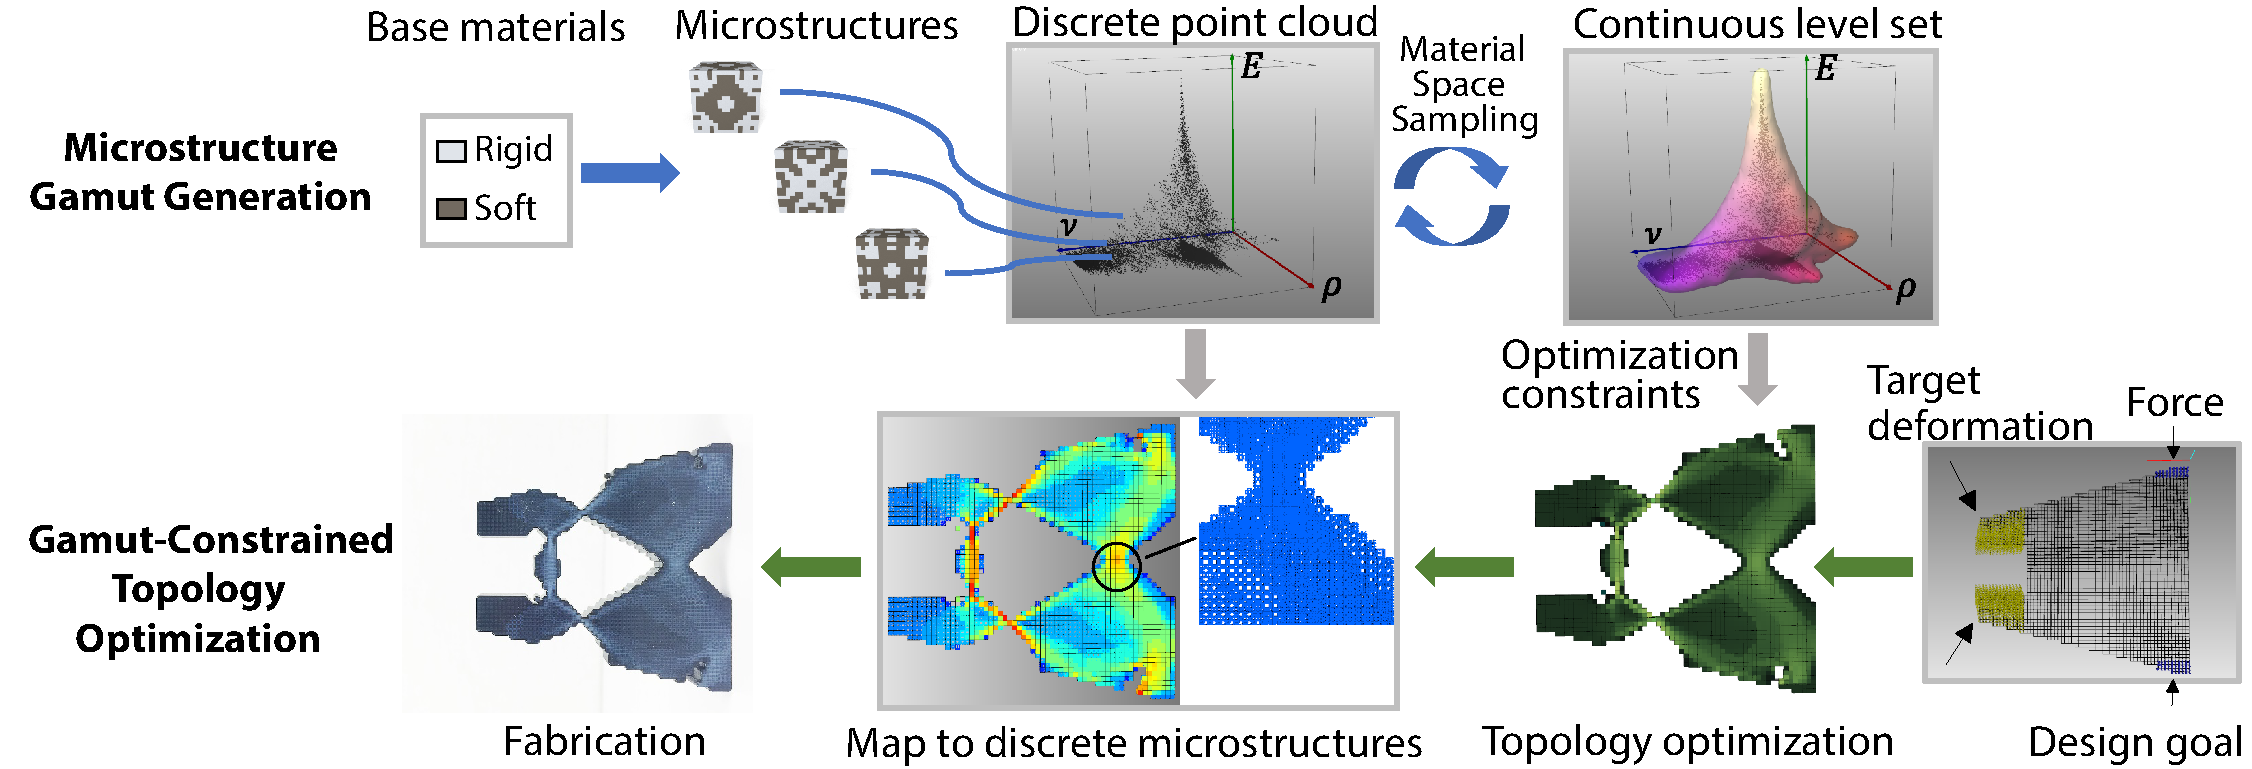
\includegraphics[width=0.95\textwidth]{images/topoptOverview.pdf}
	\caption{Inverse design algorithm.}
	\label{fig:topoptOverview}
\end{figure}
\subsection{Gamut Exploration}
In the first stage, we estimate the gamut of material properties covered by all possible microstructures made by spatial arrangement of base materials. 
Since exhaustively computing the properties of all these microstructures is, in practice, intractable, we progressively increase the material space by alternating a stochastic search and a continuous optimization. The first step introduces discrete changes in the materials of the microstructures and allows emergence of new types of microstructures. The second step allows to locally push the material space boundaries by refining the microstructure shapes. After completing this stage, we obtain a discrete representation of the space of material properties and the mapping between these properties and the corresponding microstructures.

\subsection{Gamut-Constrained Topology Optimization}
In the second stage, we construct a smooth continuous gamut representation of the material property space by using a level set field. We define our topology optimization problem directly in this space. Our approach minimizes the objective function over possible material parameters while asking for strict satisfaction of the physics constraints -- typically, the static equilibrium -- as well as the strict satisfaction of the physical parameter bounds. Taking advantage of our gamut representation as a level set, we formulate this last constraint as limiting the material properties to stay on the negative side of the level set. This guarantees that the material properties that we use in the optimization are always physically realizable.


\subsection{Discovering Families of Extremal Structures}
\begin{figure}[ht]
	\centering
	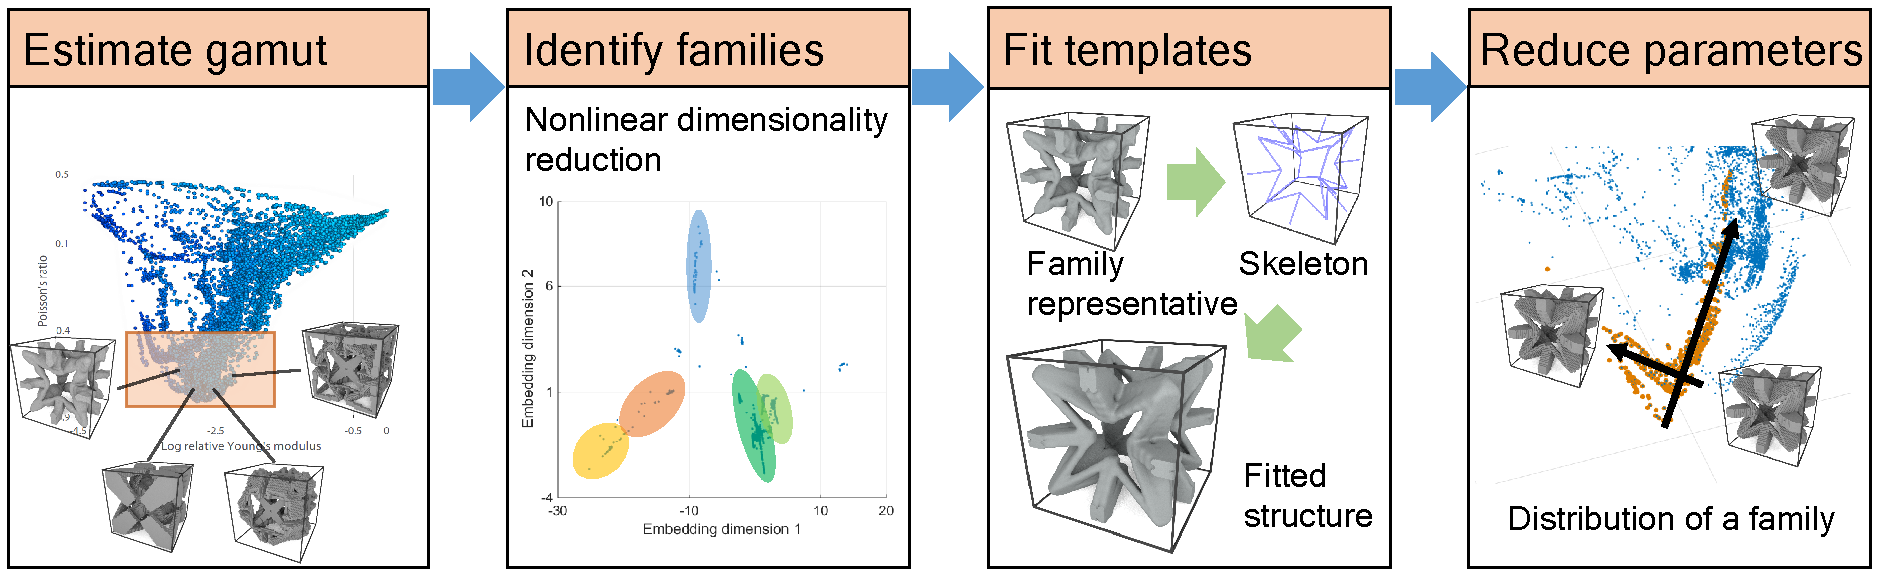
\includegraphics[width=0.9\textwidth]{images/discoverPipe.pdf}
	\caption{A computational process for discovery of extremal microstructure families. Given a set of physical properties and design constraints, we estimate the material property gamut using stochastic sampling and topology optimization. Structures near the gamut boundary are grouped into families using nonlinear dimensionality reduction. A representative from each family is fitted with a template represented as a skeleton. Beams are placed on the skeleton edges with optimized parameters to fit the original structure. Structure variations with the same topology can be generated by varying the beam parameters. Finally, reduced template parameters are computed to reveal domain-specific design principles}
	\label{fig:discoverFamily}
\end{figure}
In addition to facilitating gamut-constrained topology optimization, 
the microstructure gamut enables discovery of 
families of structures with extremal physical properties.
Our discovery pipeline has four steps (Figure~\ref{fig:discoverFamily}).
The first step estimates the material property gamut, which is the range of material properties achieved by microstructures. Here a microstructure is defined on a 3D regular grid composed of hexahedral voxels. The design space includes all possible material assignments to the voxels. Since exhaustively simulating all possible microstructures is impractical, this step computes a set of sample microstructures. The sampling algorithm alternates between topology optimization and stochastic discrete search to progressively expand the gamut~\cite{Zhu2017}. The topology optimization stage pushes structures towards outside of the gamut boundary along gradient directions. The stochastic stage introduces discrete changes to escape local optima.

In the second step, common geometric traits are identified among microstructures near the gamut boundary. Geometrically similar structures are grouped into families using nonlinear dimensionality reduction (NLDR). Isomap~\cite{tenenbaum2000global} is used as the reduction method because it can discover long sequences of related structures while keeping distant points separated. The effectiveness of NLDR depends on the distance metric that measures geometric difference. A smoothed Euclidean norm is chosen for robustness (figure S1). NLDR outputs an embedding of the microstructures in a low-dimensional space where similar structures are closely packed. Microstructures in the embedding space are clustered using a Gaussian mixture model~\cite{mclachlan2007algorithm} where each cluster corresponds to a family. Families with a significant number ($\geq 200$) of members are extracted for further analysis.

The third step in our process constructs templates for each microstructure family. We observe that most of the extremal structures are composed from beams, plates and blocks. All of these structures can be represented as cuboids with different edge lengths. We therefore chose cuboids as the building blocks for microstructure templates, and note that some structures near the boundary do not fit the cuboid representation (figure. S4).
To find a template from a family representative, its topology is computed using a morphological skeleton~\cite{Lee1994Skel}.
The morphological skeleton is a set of connected edges that largely preserves topological and branching characteristics of the structures. The skeleton is converted into a graph in order to represent a template. A cuboid is placed on each edge of the graph with optimized sizing and orientation to best match the representative structure. More details of the process are available in the supplementary text.

Finally, reduced parameters are computed to allow an intuitive navigation in the material property space. Since the templates from the previous step contain tens of parameters that do not directly correspond to material properties, it is still difficult to understand the key design principles. The reduced parameters allow for direct tuning of each material property. For a given parametric template, its parameters are fitted to all structures of the corresponding family. Principal component regression (PCR) is then performed on the set of fitted template parameters to find principal directions in the template parameters space. Varying the parameters in a direction corresponds to moving on the gamut boundary in a certain direction. A reduced parameter is assigned to each direction to control amount of change along that direction.
\section{Coarsening for Dynamics}
The realistic simulation of highly-dynamic elastic objects is important for a broad range of applications in computer graphics, engineering and computational fabrication.
However, whether simulating flipping toys, jumping robots, prosthetics or quickly moving creatures, performing such simulations in the presence of contact, impact and friction is both time consuming and inaccurate.
We propose Dynamics-Aware Coarsening (DAC) and the Boundary Balanced Impact (BBI) model for the accurate simulation of dynamic, elastic objects undergoing both large scale deformation and frictional contact.
Our methods aim to balance efficiency and accuracy to enable design-for-fabrication optimization. They can be used for both fast, realistic animation and engineering analysis. 

We begin by observing that \emph{coarsening} offers an exciting alternative for efficient yet predictive FE modeling.
Analytical solutions for coarsening have been developed for linear material models (models where the stress varies linearly with strain)~\cite{Kharevych2009,Nesme2009,Torres:2016:HIC}.
Due to this linear assumption, and similarly to the linear modal models discussed above, we find them difficult to apply for the accurate modeling of the nonlinear materials required for 3D-printed objects.
Even though our proposed DDFEM overcomes the linear limitation of prior work, it does not account for dynamic effects, inertial properties, nor material damping characteristics.


\bibliographystyle{plain}
\bibliography{proposal}
\end{document}